\subsection{GPU Accelerating \textit{k}mer Counting}
While different GPU accelerated \textit{k}mer counting solutions such as Gerbil \cite{gerbil} have been developed in previous work, we opted to develop our own \textit{k}mer counting method because the \textit{k}mer counting problem solved in KAGE is slightly different than the typical \textit{k}mer counting problem described in section \ref{background:kmers_and_the_kmer_counting_problem}.
Rather than counting the frequency of every observed \textit{k}mer in the input reads, or even the frequency of every observed \textit{k}mer where the frequency is larger than some threshold, KAGE is only interested in counting the observed frequencies for a predetermined set of \textit{k}mers.
This revised problem is easier to solve in practice because the memory constraints are significantly less.
In the interest of brevity, we will refer to the typical \textit{k}mer counting problem described section \ref{background:kmers_and_the_kmer_counting_problem} as \textit{full kmer counting}, and the simpler problem where we only count the frequencies of a predetermined set of \textit{k}mers as \textit{partial kmer counting} \ref{methods:gpu_accelerating_kmer_counting:partial_kmer_counting}.

\definecolor{kmer1}{RGB}{40,40,215}
\definecolor{kmer2}{RGB}{0,150,0}
\definecolor{kmer3}{RGB}{225,30,30}
\definecolor{kmer4}{RGB}{20,150,150}

\begin{figure}[H]
\begin{center}
\scalebox{1}{
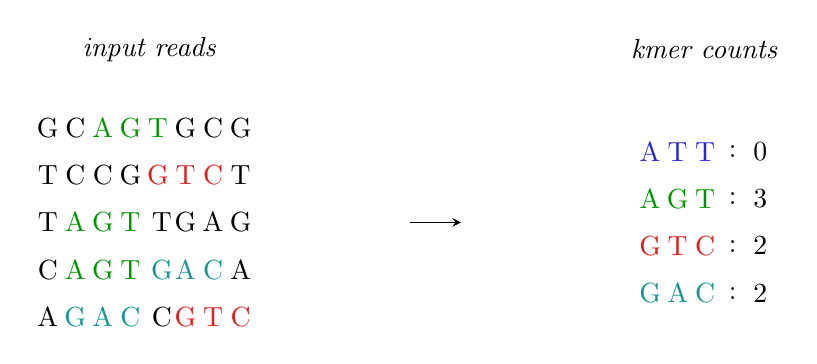
\begin{tikzpicture}
  % titles
  \node at(-0.55,3)(){\textit{input reads}};
  % read 1
  \node at(-1.85,2){G};
  \node at(-1.5,2){C};
  \node at(-1.15,2){\textcolor{kmer2}{A}};
  \node at(-.8,2){\textcolor{kmer2}{G}};
  \node at(-.45,2){\textcolor{kmer2}{T}};
  \node at(-.1,2){G};
  \node at(.25,2){C};
  \node at(.6,2){G};
  % read 2 
  \node at(-1.85,1.4){T};
  \node at(-1.5,1.4){C};
  \node at(-1.15,1.4){C};
  \node at(-.8,1.4){G};
  \node at(-.45,1.4){\textcolor{kmer3}{G}};
  \node at(-.1,1.4){\textcolor{kmer3}{T}};
  \node at(.25,1.4){\textcolor{kmer3}{C}};
  \node at(.6,1.4){T};
  % read 3 
  \node at(-1.85,.8){T};
  \node at(-1.5,.8){\textcolor{kmer2}{A}};
  \node at(-1.15,.8){\textcolor{kmer2}{G}};
  \node at(-.8,.8){\textcolor{kmer2}{T}};
  \node at(-.4,.8){T};
  \node at(-.1,.8){G};
  \node at(.25,.8){A};
  \node at(.6,.8){G};
  % read 4 
  \node at(-1.85,.2){C};
  \node at(-1.5,.2){\textcolor{kmer2}{A}};
  \node at(-1.15,.2){\textcolor{kmer2}{G}};
  \node at(-.8,.2){\textcolor{kmer2}{T}};
  \node at(-.4,.2){\textcolor{kmer4}{G}};
  \node at(-.1,.2){\textcolor{kmer4}{A}};
  \node at(.25,.2){\textcolor{kmer4}{C}};
  \node at(.6,.2){A};
  % read 5 
  \node at(-1.85,-.4){A};
  \node at(-1.5,-.4){\textcolor{kmer4}{G}};
  \node at(-1.15,-.4){\textcolor{kmer4}{A}};
  \node at(-.8,-.4){\textcolor{kmer4}{C}};
  \node at(-.4,-.4){C};
  \node at(-.1,-.4){\textcolor{kmer3}{G}};
  \node at(.25,-.4){\textcolor{kmer3}{T}};
  \node at(.6,-.4){\textcolor{kmer3}{C}};
  % Arrow
  \draw [-stealth](2.75,.8) -- (3.4,.8);
  % k-mer counts
  \node at(6.5,3)(){\textit{kmer counts}};
  % k-mer 1
  \node at(5.8,1.7){\textcolor{kmer1}{A}};
  \node at(6.15,1.7){\textcolor{kmer1}{T}};
  \node at(6.5,1.7){\textcolor{kmer1}{T}};
  \node at(6.85,1.7){:};
  \node at(7.2,1.7){0};
  % k-mer 2 
  \node at(5.8,1.1){\textcolor{kmer2}{A}};
  \node at(6.15,1.1){\textcolor{kmer2}{G}};
  \node at(6.5,1.1){\textcolor{kmer2}{T}};
  \node at(6.85,1.1){:};
  \node at(7.2,1.1){3};
  % k-mer 3 
  \node at(5.8,.5){\textcolor{kmer3}{G}};
  \node at(6.15,.5){\textcolor{kmer3}{T}};
  \node at(6.5,.5){\textcolor{kmer3}{C}};
  \node at(6.85,.5){:};
  \node at(7.2,.5){2};
  % k-mer 4 
  \node at(5.8,-.1){\textcolor{kmer4}{G}};
  \node at(6.15,-.1){\textcolor{kmer4}{A}};
  \node at(6.5,-.1){\textcolor{kmer4}{C}};
  \node at(6.85,-.1){:};
  \node at(7.2,-.1){2};
\end{tikzpicture}
}
\caption{
  In KAGE, we are only interested in counting the observed frequencies of a predefined set of \textit{k}mers, as opposed to every observed \textit{k}mer in the sequenced reads.
}
\label{methods:gpu_accelerating_kmer_counting:partial_kmer_counting}
\end{center}
\end{figure}

\subsubsection{Method 2: Parallel GPU Hash Table implemented in CUDA}
Our next attempt at GPU accelerating \textit{k}mer counting was to implement our own GPU accelerated hash table in native CUDA, which is Nvidia's programming platform \ref{background:graphical_processing_units:programming_model_and_cuda}.
This would grant us much granular control over our implementation compared to the method described in section \ref{methods:initial_testing} where we constrained ourself to using CuPy's function interface.

\textbf{\large{Implementation}}

Unlike the hash table used in the previous method, this hash table uses a simpler open addressing with linear probing scheme for insertions, updates and queries.
The hash table data structure is thus a simple structure of arrays, with one array constituting the hash table keys and another the associated values (counts).
It is implemented in CUDA as a C++ class and supports the following functionalities:
\begin{compactitem}
  \item key insertion: only performed once upon initialization.
  \item key counting: for each key, if it exists in the hash table, increment the associated hash table value by one.
  \item key querying: for each key, if it exists in the hash table, fetch the associated hash table value.
\end{compactitem}

Each of these methods are implemented using custom CUDA kernels, allowing for each operation to happen for a large number of \textit{k}mers in parallel on the GPU.
Thus, the insertion, counting and query implementations all expect arrays of \textit{k}mers where a single CUDA thread is assigned to each \textit{k}mer to fulfill the insertion, count update or query.

\textbf{Hashing and Probing Scheme}

All of the kernels implemented for this hash table solution share the same linear probing scheme to resolve collisions.
Thus, when a CUDA thread is assigned a \textit{k}mer $k$ from the input array (either for insertion, count updating or querying), it will perform a murmur hash (cite murmur) to find the initial probe position $p_0$ in the hash table.

\definecolor{misscolor}{RGB}{255,215,215}
\definecolor{hitcolor}{RGB}{215,255,215}
\definecolor{countcolor}{RGB}{240,240,240}

\begin{figure}[H]
\begin{center}
\scalebox{1}{
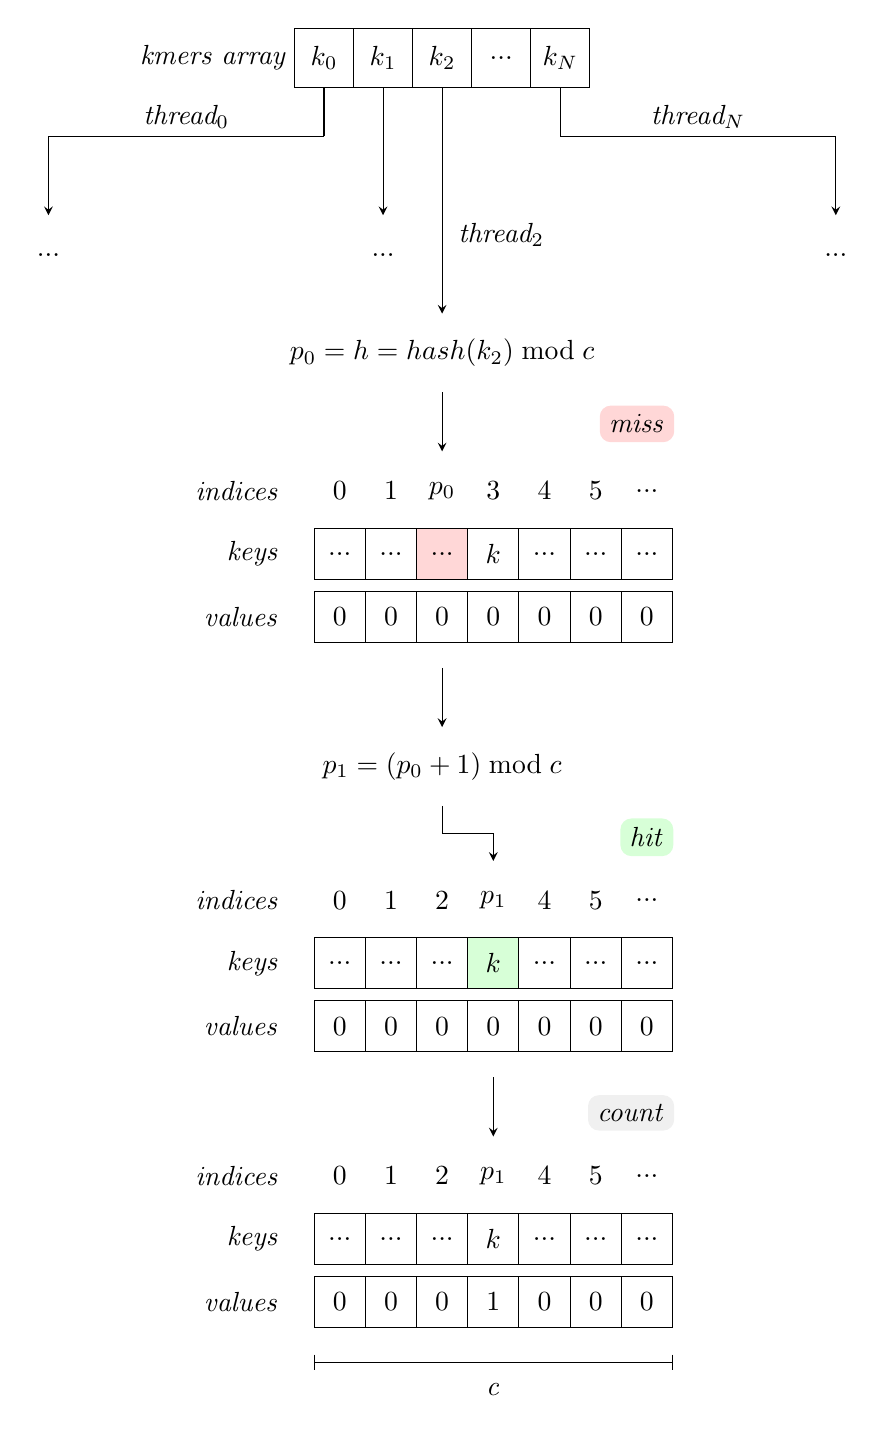
\begin{tikzpicture}
  % in kmers
  \node at(-2.9,0)(){\textit{\smaller{kmers array}}};
  \node at(-1.5,0)[draw,minimum width=0.75cm,minimum height=0.75cm](k0){\smaller{$k_0$}};
  \node at(-.75,0)[draw,minimum width=0.75cm,minimum height=0.75cm](k1){\smaller{$k_1$}};
  \node at(0,0)[draw,minimum width=0.75cm,minimum height=0.75cm](k2){\smaller{$k_2$}};
  \node at(.75,0)[draw,minimum width=0.75cm,minimum height=0.75cm](gap){\smaller{$...$}};
  \node at(1.5,0)[draw,minimum width=0.75cm,minimum height=0.75cm](kn){\smaller{$k_N$}};
  % CUDA threads
  % k0
  \draw [](k0) -- (-1.5,-1);
  \draw [](-1.5,-1) -- (-5,-1);
  \draw [-stealth](-5,-1) -- (-5,-2);
  \node at(-3.25,-.75)(){\textit{\smaller{thread$_0$}}};
  \node at(-5,-2.5)(){...};
  % k1
  \draw [-stealth](k1) -- (-.75,-2);
  \node at(-.75,-2.5)(){...};
  % kn
  \draw [](kn) -- (1.5,-1);
  \draw [](1.5,-1) -- (5,-1);
  \draw [-stealth](5,-1) -- (5,-2);
  \node at(3.25,-.75)(){\textit{\smaller{thread$_N$}}};
  \node at(5,-2.5)(){...};
  % k2
  \draw [-stealth](k2) -- (0,-3.25);
  \node at(.75,-2.25)(){\textit{\smaller{thread$_2$}}};
  % hash
  \node at(0,-3.75)(){\smaller{\textit{$p_0=h=hash(k_2) \bmod c$}}};
  % probe 1
  \draw [-stealth](0,-4.25) -- (0,-5);
  \node at(2.475,-4.65)[fill=misscolor,rounded corners](){\textit{\smaller{miss}}};
  % titles
  \node at(-2.6,-5.5)(){\textit{\smaller{indices}}};
  \node at(-2.4,-6.3)(){\textit{\smaller{keys}}};
  \node at(-2.55,-7.1)(){\textit{\smaller{values}}};
  % indices
  \node at(-1.3,-5.5)[minimum width=0.65cm,minimum height=0.65cm](){\smaller{$0$}};
  \node at(-.65,-5.5)[minimum width=0.65cm,minimum height=0.65cm](){\smaller{$1$}};
  \node at(0,-5.5)[minimum width=0.65cm,minimum height=0.65cm](){\smaller{$p_0$}};
  \node at(.65,-5.5)[minimum width=0.65cm,minimum height=0.65cm](){\smaller{$3$}};
  \node at(1.3,-5.5)[minimum width=0.65cm,minimum height=0.65cm](){\smaller{$4$}};
  \node at(1.95,-5.5)[minimum width=0.65cm,minimum height=0.65cm](){\smaller{$5$}};
  \node at(2.6,-5.5)[minimum width=0.65cm,minimum height=0.65cm](){\smaller{$...$}};
  % keys
  \node at(-1.3,-6.3)[draw,minimum width=0.65cm,minimum height=0.65cm](){\smaller{$...$}};
  \node at(-.65,-6.3)[draw,minimum width=0.65cm,minimum height=0.65cm](){\smaller{$...$}};
  \node at(0,-6.3)[draw,minimum width=0.65cm,minimum height=0.65cm,fill=misscolor](){\smaller{$...$}};
  \node at(.65,-6.3)[draw,minimum width=0.65cm,minimum height=0.65cm](){\smaller{$k$}};
  \node at(1.3,-6.3)[draw,minimum width=0.65cm,minimum height=0.65cm](){\smaller{$...$}};
  \node at(1.95,-6.3)[draw,minimum width=0.65cm,minimum height=0.65cm](){\smaller{$...$}};
  \node at(2.6,-6.3)[draw,minimum width=0.65cm,minimum height=0.65cm](){\smaller{$...$}};
  % values
  \node at(-1.3,-7.1)[draw,minimum width=0.65cm,minimum height=0.65cm](){\smaller{$0$}};
  \node at(-.65,-7.1)[draw,minimum width=0.65cm,minimum height=0.65cm](){\smaller{$0$}};
  \node at(0,-7.1)[draw,minimum width=0.65cm,minimum height=0.65cm](){\smaller{$0$}};
  \node at(.65,-7.1)[draw,minimum width=0.65cm,minimum height=0.65cm](){\smaller{$0$}};
  \node at(1.3,-7.1)[draw,minimum width=0.65cm,minimum height=0.65cm](){\smaller{$0$}};
  \node at(1.95,-7.1)[draw,minimum width=0.65cm,minimum height=0.65cm](){\smaller{$0$}};
  \node at(2.6,-7.1)[draw,minimum width=0.65cm,minimum height=0.65cm](){\smaller{$0$}};
  % probe 2
  \draw [-stealth](0,-7.75) -- (0,-8.5);
  \node at(0,-9)(){\smaller{\textit{$p_1=(p_0 + 1) \bmod c$}}};
  \draw [](0,-9.5) -- (0,-9.85);
  \draw [](0,-9.85) -- (.65,-9.85);
  \draw [-stealth](.65,-9.85) -- (.65,-10.2);
  \node at(-2.6,-10.7)(){\textit{\smaller{indices}}};
  \node at(-2.4,-11.5)(){\textit{\smaller{keys}}};
  \node at(-2.55,-12.3)(){\textit{\smaller{values}}};
  \node at(2.6,-9.9)[fill=hitcolor,rounded corners](){\textit{\smaller{hit}}};
  % indices
  \node at(-1.3,-10.7)[minimum width=0.65cm,minimum height=0.65cm](){\smaller{$0$}};
  \node at(-.65,-10.7)[minimum width=0.65cm,minimum height=0.65cm](){\smaller{$1$}};
  \node at(0,-10.7)[minimum width=0.65cm,minimum height=0.65cm](){\smaller{$2$}};
  \node at(.65,-10.7)[minimum width=0.65cm,minimum height=0.65cm](){\smaller{$p_1$}};
  \node at(1.3,-10.7)[minimum width=0.65cm,minimum height=0.65cm](){\smaller{$4$}};
  \node at(1.95,-10.7)[minimum width=0.65cm,minimum height=0.65cm](){\smaller{$5$}};
  \node at(2.6,-10.7)[minimum width=0.65cm,minimum height=0.65cm](){\smaller{$...$}};
  % keys
  \node at(-1.3,-11.5)[draw,minimum width=0.65cm,minimum height=0.65cm](){\smaller{$...$}};
  \node at(-.65,-11.5)[draw,minimum width=0.65cm,minimum height=0.65cm](){\smaller{$...$}};
  \node at(0,-11.5)[draw,minimum width=0.65cm,minimum height=0.65cm](){\smaller{$...$}};
  \node at(.65,-11.5)[draw,minimum width=0.65cm,minimum height=0.65cm,fill=hitcolor](){\smaller{$k$}};
  \node at(1.3,-11.5)[draw,minimum width=0.65cm,minimum height=0.65cm](){\smaller{$...$}};
  \node at(1.95,-11.5)[draw,minimum width=0.65cm,minimum height=0.65cm](){\smaller{$...$}};
  \node at(2.6,-11.5)[draw,minimum width=0.65cm,minimum height=0.65cm](){\smaller{$...$}};
  % values
  \node at(-1.3,-12.3)[draw,minimum width=0.65cm,minimum height=0.65cm](){\smaller{$0$}};
  \node at(-.65,-12.3)[draw,minimum width=0.65cm,minimum height=0.65cm](){\smaller{$0$}};
  \node at(0,-12.3)[draw,minimum width=0.65cm,minimum height=0.65cm](){\smaller{$0$}};
  \node at(.65,-12.3)[draw,minimum width=0.65cm,minimum height=0.65cm](){\smaller{$0$}};
  \node at(1.3,-12.3)[draw,minimum width=0.65cm,minimum height=0.65cm](){\smaller{$0$}};
  \node at(1.95,-12.3)[draw,minimum width=0.65cm,minimum height=0.65cm](){\smaller{$0$}};
  \node at(2.6,-12.3)[draw,minimum width=0.65cm,minimum height=0.65cm](){\smaller{$0$}};
  % count
  \draw [-stealth](.65,-12.95) -- (.65,-13.7);
  \node at(-2.6,-14.2)(){\textit{\smaller{indices}}};
  \node at(-2.4,-15)(){\textit{\smaller{keys}}};
  \node at(-2.55,-15.8)(){\textit{\smaller{values}}};
  \node at(2.4,-13.4)[fill=countcolor,rounded corners](){\textit{\smaller{count}}};
  % indices
  \node at(-1.3,-14.2)[minimum width=0.65cm,minimum height=0.65cm](){\smaller{$0$}};
  \node at(-.65,-14.2)[minimum width=0.65cm,minimum height=0.65cm](){\smaller{$1$}};
  \node at(0,-14.2)[minimum width=0.65cm,minimum height=0.65cm](){\smaller{$2$}};
  \node at(.65,-14.2)[minimum width=0.65cm,minimum height=0.65cm](){\smaller{$p_1$}};
  \node at(1.3,-14.2)[minimum width=0.65cm,minimum height=0.65cm](){\smaller{$4$}};
  \node at(1.95,-14.2)[minimum width=0.65cm,minimum height=0.65cm](){\smaller{$5$}};
  \node at(2.6,-14.2)[minimum width=0.65cm,minimum height=0.65cm](){\smaller{$...$}};
  % keys
  \node at(-1.3,-15)[draw,minimum width=0.65cm,minimum height=0.65cm](){\smaller{$...$}};
  \node at(-.65,-15)[draw,minimum width=0.65cm,minimum height=0.65cm](){\smaller{$...$}};
  \node at(0,-15)[draw,minimum width=0.65cm,minimum height=0.65cm](){\smaller{$...$}};
  \node at(.65,-15)[draw,minimum width=0.65cm,minimum height=0.65cm](){\smaller{$k$}};
  \node at(1.3,-15)[draw,minimum width=0.65cm,minimum height=0.65cm](){\smaller{$...$}};
  \node at(1.95,-15)[draw,minimum width=0.65cm,minimum height=0.65cm](){\smaller{$...$}};
  \node at(2.6,-15)[draw,minimum width=0.65cm,minimum height=0.65cm](){\smaller{$...$}};
  % values
  \node at(-1.3,-15.8)[draw,minimum width=0.65cm,minimum height=0.65cm](){\smaller{$0$}};
  \node at(-.65,-15.8)[draw,minimum width=0.65cm,minimum height=0.65cm](){\smaller{$0$}};
  \node at(0,-15.8)[draw,minimum width=0.65cm,minimum height=0.65cm](){\smaller{$0$}};
  \node at(.65,-15.8)[draw,minimum width=0.65cm,minimum height=0.65cm](){\smaller{$1$}};
  \node at(1.3,-15.8)[draw,minimum width=0.65cm,minimum height=0.65cm](){\smaller{$0$}};
  \node at(1.95,-15.8)[draw,minimum width=0.65cm,minimum height=0.65cm](){\smaller{$0$}};
  \node at(2.6,-15.8)[draw,minimum width=0.65cm,minimum height=0.65cm](){\smaller{$0$}};
  % capacity
  \draw [](-1.625,-16.57) -- (2.925,-16.57); % -16.57
  \draw [](-1.625,-16.47) -- (-1.625,-16.67); % -16.47, -16.67
  \draw [](2.925,-16.47) -- (2.925,-16.67);
  \node at(.65,-16.92)(c){\smaller{\textit{c}}};
\end{tikzpicture}
}
\caption{
  As an array of \textit{N} 64-bit integer encoded kmers are counted by the hash table, \textit{N} CUDA threads will launch and each will compute the first probe position $p_0$ for its assigned kmer \textit{k}. Then, if the key at slot $p_0$ does not contain \textit{k}, it will continue probing by linearly moving up to the next consecutive slot until either an empty key or \textit{k} observed. If an empty key is observed, the thread terminates without changing any of the hash table's values. If \textit{k} is observed, the current slot's value is incremented.
}
\label{methods:gpu_accelerating_kmer_counting:method2:figures:probing_scheme}
\end{center}
\end{figure}

\textbf{Insertions}

...

\subsubsection{Method 3: Parallel GPU Hash Table without CUDA or C++}
...

\subsection{GPU Accelerating \textit{k}mer Hashing}

